% !TEX TS-program = LuaLaTeX
% Gemini theme
% https://github.com/anishathalye/gemini

\documentclass[final]{beamer}

% ====================
% Packages
% ====================

%\usepackage[T1]{fontenc}
\usepackage{lmodern}
\usepackage[size=custom,width=106.7,height=80.0,scale=0.85]{beamerposter}% max=135x76
\usetheme{gemini}
\usecolortheme{gemini}
\usepackage{graphicx}
\usepackage{amsmath}
\usepackage{amsfonts,amssymb,latexsym,amscd}
\usepackage[numbers]{natbib}
\usepackage{amsmath}
\usepackage{booktabs}
\usepackage{tikz}
\usepackage{pgfplots}
\usepackage{comment}
\usepackage{scalefnt}
\usepackage{isomath}
\usepackage{subfig}
\usepackage{bm}
\usepackage{multirow}
\usepackage{microtype}
\usepackage{tikz}

\usetikzlibrary{calc,patterns,decorations.pathmorphing,decorations.markings,decorations.pathreplacing}
\usetikzlibrary{shapes,fit}
\usetikzlibrary{positioning}
\usetikzlibrary{decorations.text}
\newcommand\independent{\protect\mathpalette{\protect\independenT}{\perp}}
\def\independenT#1#2{\mathrel{\rlap{$#1#2$}\mkern2mu{#1#2}}}
\newcommand*{\og}{\textcolor{orange}}
\usepackage{listings}
\def\listingsfont{\ttfamily}

\graphicspath{{./Figures/}}
\newcommand{\indep}{\rotatebox[origin=c]{90}{$\models$}}

%TIKZ
\usepackage{tikz}
\usetikzlibrary{shapes.geometric, arrows}

\tikzstyle{startstop} = [circle, minimum size=2.5cm, text centered, draw=black, fill=green!30]
\tikzstyle{process} = [rectangle, rounded corners, minimum width=2cm, minimum height=1cm, text centered, draw=black, fill=yellow!50]
\tikzstyle{decision} = [circle, minimum size=2.5cm, text centered, draw=black, fill=red!30]
\tikzstyle{arrow} = [thick, ->, >=stealth, line width=0.5mm, scale=2]
\tikzstyle{process2} = [circle, minimum size=2.5cm, text centered, draw=black, fill=yellow!50]
\tikzstyle{end} = [circle, minimum size=2.5cm, text centered, draw=black, fill=cyan!30]
%TIKZ



%%%%%%%%%
%Beambox
%%%%%%%%%
%\setbeamertemplate{blocks}[rounded][shadow=true]
\definecolor{cl_postit}{RGB}{255,255,136}
\setbeamercolor{postit}{fg=black,bg=cl_postit}
\newcommand{\source}[1]{\begin{textblock*}{8cm}(7.95cm,7.7cm)
    \begin{beamercolorbox}[ht=0.5cm,right]{framesource}
        \usebeamerfont{framesource}\usebeamercolor[fg]{framesource} [{#1}]
    \end{beamercolorbox}
\end{textblock*}}
% ====================
% Lengths
% ====================

% If you have N columns, choose \sepwidth and \colwidth such that
% (N+1)*\sepwidth + N*\colwidth = \paperwidth
\newlength{\sepwidth}
\newlength{\colwidth}
\setlength{\sepwidth}{0.025\paperwidth}
\setlength{\colwidth}{0.3\paperwidth}

\newcommand{\separatorcolumn}{\begin{column}{\sepwidth}\end{column}}

  
% ====================
% Title
% ====================

\title{Implementation of a probabilistic Softmax for BNNs (Group 11)}
\logoleft{%
%
\includegraphics[width=0.06\paperwidth]{Figures/Polytechnique_logo.pdf}
}
\logoright{%
}
%\author{Adapted from the work proposed by Nguyen \& Goulet \quad  David Wardan, Khalil Sabri, \,and\, Miquel Florensa  -- Polytechnique Montr\'{e}al, Canada}
\author{  David Wardan, Khalil Sabri, \,and\, Miquel Florensa  -- Polytechnique Montr\'{e}al, Canada \\ \vspace{5mm} \Large Based on the work proposed by J-A. Goulet \& L. H. Nguyen}

\institute[shortinst]{}

%% ====================
%% Footer (optional)
%% ====================
%
\footercontent{
%  \href{https://www.example.com}{https://www.example.com} \hfill
  IFT6269 Project Poster 2024 } 
%  \href{mailto:alyssa.p.hacker@example.com}{alyssa.p.hacker@example.com}}


% ====================
% Body
% ====================

\begin{document}
\begin{frame}[t]

\begin{columns}
%%%%%%%%%%
%%% Column 1
%%%%%%%%%%
\begin{column}[T]{.31\textwidth}

%% Motivation
\begin{alertblock}{\Large Tractable Approximate Gaussian Inference (TAGI)}
\vspace{4pt}
\begin{columns}
\begin{column}{.5\textwidth}\vspace{23pt}
\centering
$$\text{Parameters}\left\{\begin{array}{rl}f(\bm\theta|\mathcal{D}) =&\displaystyle \frac{f(\mathcal{D}|\bm\theta)\,f(\bm\theta)}{f(\mathcal{D})}\\[25pt]
=&\mathcal{N}\big(\bm{\theta};\bm{\mu}_{\bm{\theta}|\mathcal{D}},\bm{\sigma}^2_{\bm{\theta}|\mathcal{D}}\mathbf{I})\end{array}\right.$$
$$\hspace{22.5mm}\begin{array}{r}\text{Hidden}\\\text{states}\end{array}\left\{\begin{array}{rl}~\\[-20pt]f(\bm{z}|\mathcal{D}) =&\mathcal{N}\big(\bm{z};\bm{\mu}_{\bm{Z}|\mathcal{D}},\bm{\sigma}^2_{\bm{Z}|\mathcal{D}}\mathbf{I})\\[-10pt]
&~\end{array}\right.$$


\alert{\bf Scalable analytical Bayesian inference\\ in any neural network architecture}
\end{column}
\begin{column}{.5\textwidth}


\begin{itemize}\setlength\itemsep{0.5em}
\item Bayesian analytical inference $\left\{\begin{array}{ll} \text{parameters}\\
\text{hidden states}\end{array}\right.$\vspace{-5.5mm}
\item Fast and scalable $\to \mathcal{O}(n)$
\item End-to-end treatment of uncertainty
\item No gradient backpropagation
\end{itemize}
\end{column}
\end{columns}\bigskip
\end{alertblock}

\vspace{-0.7cm}

\begin{block}{TAGI - Forward uncertainty propagation}
 \begin{figure}[h!]
 \centering
  
\includegraphics[width=1\textwidth]{Figures/forward_pass.pdf}
 \end{figure}

 \begin{columns}
 \begin{column}{0.33\textwidth}
\begin{equation*} \label{eq:nn}
\begin{split}
\bm{z}^{(1)} &= \bm{w}^{(0)} \bm{x} + \bm{b}^{(0)}, \\
\bm{a}^{(i)} &= {\color{cyan}\tilde{\sigma}(\bm{z}^{(i)})}, \\
\bm{z}^{(i)} &= {\color{magenta}\bm{w}^{(i)} \bm{a}^{(i-1)}} + \bm{b}^{(i)}, \\
\bm{z}^{(\mathtt{O})} &=  {\color{magenta}\bm{w}^{(\mathtt{L})} \bm{a}^{(\mathtt{L})}} + \bm{w}^{(\mathtt{L})} \\
\bm{y} &=  \bm{z}^{(\mathtt{O})} + \bm{v}.
\end{split}
\end{equation*} 
\ \ where $\bm{v}$ are the observation \\ \ \ noise.
\end{column}

\begin{column}{0.33\textwidth}
\ \ \ \ \ \ \ \ \ \ \ \ \ \ {\color{magenta}Challenge 1:} GMA
\vspace{1.1cm}
 \begin{figure}[h!]
 \centering
  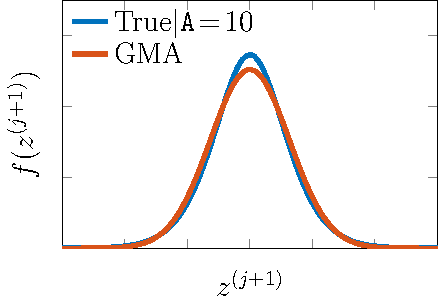
\includegraphics[width=0.85\textwidth]{Figures/GMA_CLT_10.pdf}
 \end{figure}
\vspace{1cm}

\end{column}
\begin{column}{0.33\textwidth}
\ \ \ \ \ {\color{cyan}Challenge 2:} Locally Linearize
 \begin{figure}[h!]
 \centering
  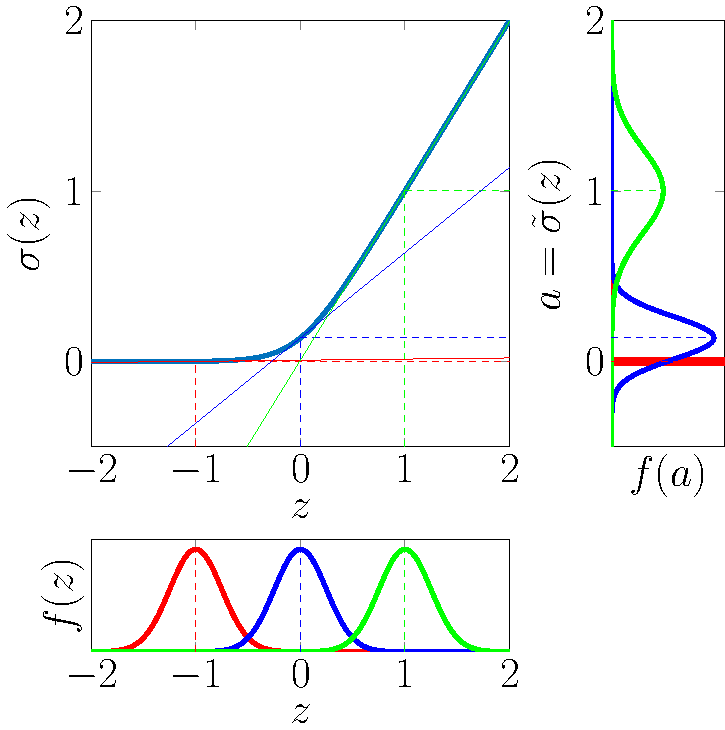
\includegraphics[width=0.8\textwidth]{Figures/Linearized_activation_fct.pdf}
 \end{figure}
\end{column}
\end{columns}
 \end{block}
 
\begin{block}{TAGI - Backward parameter and hidden state inference}
  \begin{figure}[h!]
 \centering
  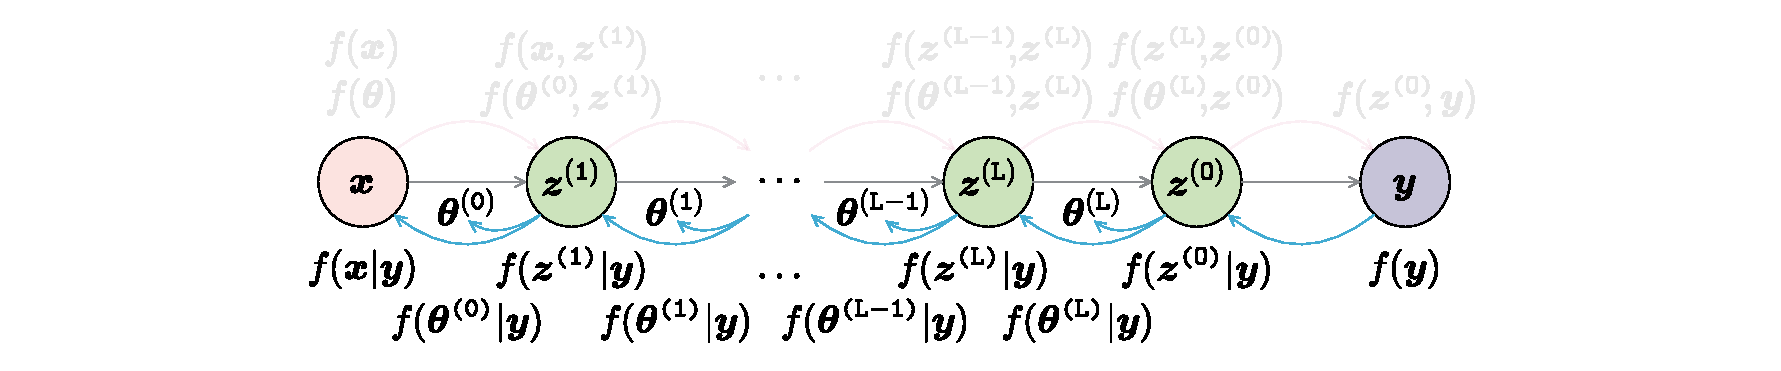
\includegraphics[width=1\textwidth]{Figures/backward_pass.pdf}
 \end{figure}


First, given the observations $\bm{y}$, the output layer is updated as
\begin{equation*} \label{eq:z0update}
\begin{split}
f\left(\boldsymbol{z}^{(\mathtt{O})} \mid \boldsymbol{y}\right) &=\mathcal{N}\left(\boldsymbol{z}^{(\mathtt{O})} ; \boldsymbol{\mu}_{\boldsymbol{Z}^{(\mathtt{O})} \mid \boldsymbol{y}}, \boldsymbol{\Sigma}_{\boldsymbol{Z}^{(\mathtt{O})} \mid \boldsymbol{y}}\right) \\
\boldsymbol{\mu}_{\boldsymbol{Z}^{(\mathtt{O})} \mid \boldsymbol{y}} &=\boldsymbol{\mu}_{\boldsymbol{Z}^{(\mathtt{O})}}+\boldsymbol{\Sigma}_{\boldsymbol{Y} \boldsymbol{Z}^{(\mathtt{O})}}^{\top} \boldsymbol{\Sigma}_{\boldsymbol{Y}}^{-1}\left(\boldsymbol{y}-\boldsymbol{\mu}_{\boldsymbol{Y}}\right) \\
\boldsymbol{\Sigma}_{\boldsymbol{Z}^{(\mathtt{O})} \mid \boldsymbol{y}} &=\boldsymbol{\Sigma}_{\boldsymbol{Z}^{(\mathtt{O})}}-\boldsymbol{\Sigma}_{\boldsymbol{Y} \boldsymbol{Z}^{(\mathtt{O})}}^{\top} \boldsymbol{\Sigma}_{\boldsymbol{Y}}^{-1} \boldsymbol{\Sigma}_{\boldsymbol{Y Z}^{(\mathtt{O})}}.
\end{split}
\end{equation*}

Next, the hidden units and parameters of the layer $i^{th}$ are updated using a layer-wise procedure as
\begin{columns}
\begin{column}{0.5\textwidth}
\begin{equation*}  \label{eq:layerwiseupdate}
\begin{split}
f(\boldsymbol{z} \mid \boldsymbol{y}) &=\mathcal{N}\left(\boldsymbol{z} ; \boldsymbol{\mu}_{\boldsymbol{Z} \mid \boldsymbol{y}}, \boldsymbol{\Sigma}_{\boldsymbol{Z} \mid \boldsymbol{y}}\right) \\
\boldsymbol{\mu}_{\boldsymbol{Z} \mid \boldsymbol{y}} &=\boldsymbol{\mu}_{\boldsymbol{Z}}+\mathbf{J}_{\boldsymbol{Z}}\left(\boldsymbol{\mu}_{\boldsymbol{Z}^{+} \mid \boldsymbol{y}}-\boldsymbol{\mu}_{\boldsymbol{Z}^{+}}\right) \\
\boldsymbol{\Sigma}_{\boldsymbol{Z} \mid \boldsymbol{y}} &=\boldsymbol{\Sigma}_{\boldsymbol{Z}}+\mathbf{J}_{\boldsymbol{Z}}\left(\boldsymbol{\Sigma}_{\boldsymbol{Z}^{+} \mid \boldsymbol{y}}-\boldsymbol{\Sigma}_{\boldsymbol{Z}^{+}}\right) \mathbf{J}_{\boldsymbol{Z}}^{\top} \\
\mathbf{J}_{\boldsymbol{Z}} &=\boldsymbol{\Sigma}_{\boldsymbol{Z Z}^{+}} \boldsymbol{\Sigma}_{\boldsymbol{Z}^{+}}^{-1},
\end{split}
\end{equation*}
\end{column}

\begin{column}{0.5\textwidth}
\begin{equation*}
\begin{split}
f(\boldsymbol{\theta} \mid \boldsymbol{y}) &=\mathcal{N}\left(\boldsymbol{\theta} ; \boldsymbol{\mu}_{\boldsymbol{\theta} \mid \boldsymbol{y}}, \boldsymbol{\Sigma}_{\boldsymbol{\theta} \mid \boldsymbol{y}}\right) \\
\boldsymbol{\mu}_{\boldsymbol{\theta} \mid \boldsymbol{y}} &=\boldsymbol{\mu}_{\boldsymbol{\theta}}+\mathbf{J}_{\boldsymbol{\theta}}\left(\boldsymbol{\mu}_{\boldsymbol{Z}^{+} \mid \boldsymbol{y}}-\boldsymbol{\mu}_{\boldsymbol{Z}^{+}}\right) \\
\boldsymbol{\Sigma}_{\boldsymbol{\theta} \mid \boldsymbol{y}} &=\boldsymbol{\Sigma}_{\boldsymbol{\theta}}+\mathbf{J}_{\boldsymbol{\theta}}\left(\boldsymbol{\Sigma}_{\boldsymbol{Z}^{+} \mid \boldsymbol{y}}-\boldsymbol{\Sigma}_{\boldsymbol{Z}^{+}}\right) \mathbf{J}_{\boldsymbol{\theta}}^{\top} \\
\mathbf{J}_{\boldsymbol{\theta}} &=\boldsymbol{\Sigma}_{\boldsymbol{\theta} Z^{+}} \boldsymbol{\Sigma}_{\boldsymbol{Z}^{+}}^{-1},
\end{split}
\end{equation*}
\end{column}
\end{columns}
where $\left\{\boldsymbol{\theta}^{+}, \boldsymbol{Z}^{+}\right\}$ is the short-hand notation of $\left\{\boldsymbol{\theta}^{(j+1)}, \boldsymbol{Z}^{(j+1)}\right\}$, and $\{\boldsymbol{\theta}, \boldsymbol{Z}\}$ is the short-hand notation of  $\left\{\boldsymbol{\theta}^{(j)}, \boldsymbol{Z}^{(j)}\right\}$.
\end{block}


\begin{block}{Regression toy example}
\begin{columns}
\begin{column}{0.5\textwidth}
  \begin{figure}[h!]
 \centering
  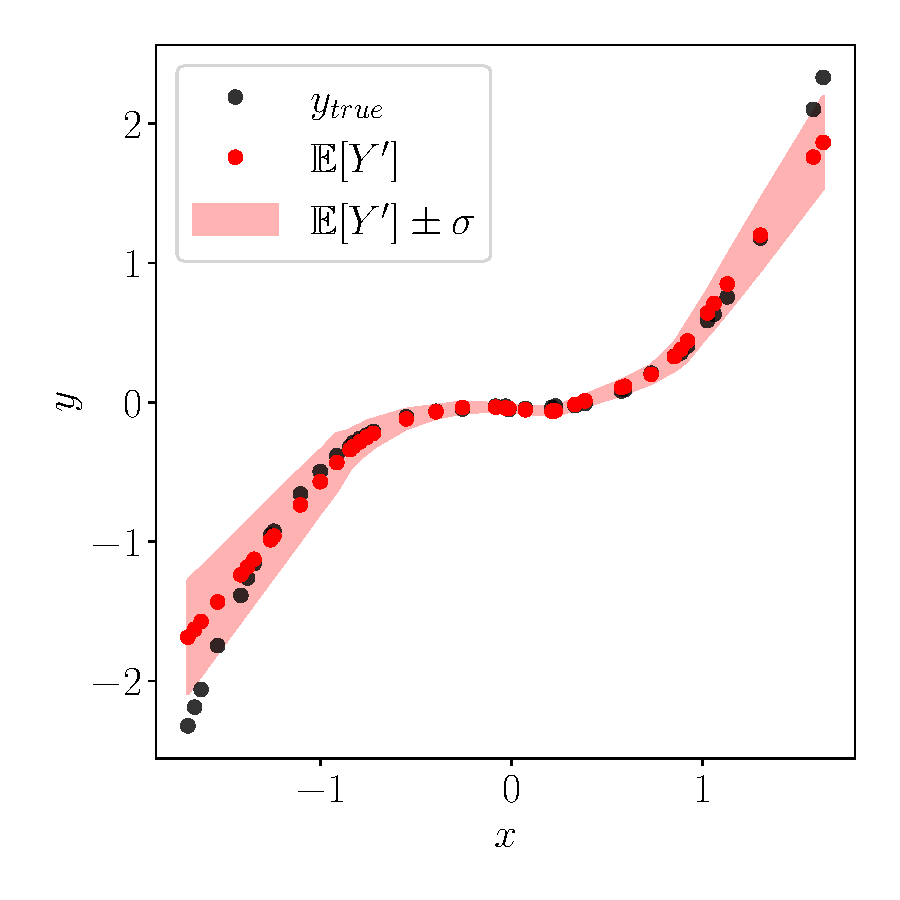
\includegraphics[width=0.8\textwidth]{Figures/toy_example.pdf}
 \end{figure}
 \end{column}
 \begin{column}{0.5\textwidth}
 \begin{itemize}
 \item We re-implement the toy example presented by the authors using the numpy library in Python.
 \item This includes defining a fully connected neural network with one layer and 40 hidden units.
 \item The figure shows the output of the model on the test set with the epistemic uncertainty.
\end{itemize}
 \end{column}
\end{columns}
\end{block}
\end{column}
%%%%%%%%%%
%%% Column 2
%%%%%%%%%%
\begin{column}[T]{.31\textwidth}

\begin{block}{Remax - Probabilistic Softmax for uncertainty propagation}\vspace{0pt}\centering

\begin{itemize}
\item TAGI cannot use directly the softmax function: $\mathtt{softmax} (\bm{z},i)= \frac{\exp (z_i)}{\sum_j \exp (z_j)}$ since $\raisebox{-1mm}{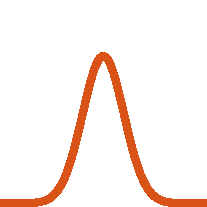
\includegraphics[height=.8cm]{distri}} / \raisebox{-1mm}{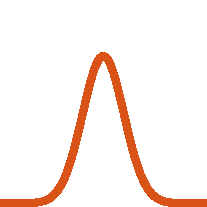
\includegraphics[height=.8cm]{distri}} \alert{\neq} \raisebox{-1mm}{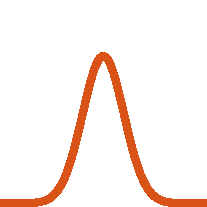
\includegraphics[height=.8cm]{distri}}. \text{ \raisebox{-2mm}{
\includegraphics[width=12mm]{cross}}}$
\item J-A. Goulet \& L. H. Nguyen propose probabilistic softmax by doing the division in log-transformed space.
\item The random variable $Z$ is Lognormal if $\ln Z$ is Normal and $\exp(Z)$ is Lognormal if $Z$ is Normal.
\item Probabilistic softmax does not work for $Z$ with high variances; $Var(Z) \approx 1$. $\text{ \raisebox{-2mm}{
\includegraphics[width=12mm]{warning}}}$
\item Alternative softmax function: $\mathtt{remax} (\bm{z},i)= \frac{\mathtt{mReLU} (z_i)}{\sum_j \mathtt{mReLU} (z_j)}$ where $\mathtt{mReLU}$ is a \textit{Mixture Rectified Linear activation Unit}.
\item We implement $\mathtt{remax}$ function in py/cuTAGI library using C++ and CUDA.
\end{itemize}



\bigskip

\begin{tikzpicture}[node distance=2cm]

% Nodes
\node (z0) [startstop] {$Z^{(\mathtt{O})}$};
\node (mrelu) [process, right of=z0, xshift=3cm] {$\mathtt{mReLU} (M)$};
\node (mtil) [process2, below of=mrelu, yshift=-2.5cm] {$\tilde{M}$};
\node (lnm) [decision, right of=mrelu, xshift=3cm] {$\ln M$};
\node (lnmtil) [decision, below of=lnm, yshift=-2.5cm] {$\ln \tilde{M}$};
\node (ahat) [decision, right of=lnm, xshift=3cm, yshift=-2.25cm] {$\check{A}$};
\node (a) [end, right of=ahat, xshift=3cm] {$A$};

% Arrows
\draw [arrow] (z0) -- (mrelu);
\draw [arrow] (mrelu) -- (lnm);
\draw [arrow] (mrelu) -- (mtil);
\draw [arrow] (mtil) -- (lnmtil);
\draw [arrow] (lnm) -- (ahat);
\draw [arrow] (lnmtil) -- (ahat);
\draw [arrow] (ahat) -- (a);

\end{tikzpicture}
\bigskip

$\begin{array}{lclll}
 {M} &=& \mathtt{mReLU}(Z^{(\mathtt{O})}) &= \mathtt{mReLU} (\raisebox{-1mm}{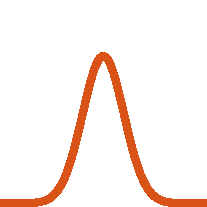
\includegraphics[height=.8cm]{distri}} ) &{ \approx \! \raisebox{-1mm}{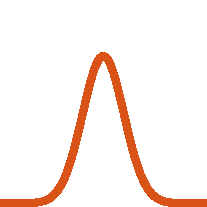
\includegraphics[height=.8cm]{distri}}}  \;{\raisebox{-0.5mm}{
\includegraphics[height=5mm]{check}}} \\[6pt]
  \tilde{M} &=& \sum_j (M_j) &=  \raisebox{-1mm}{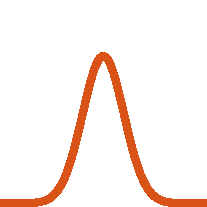
\includegraphics[height=.8cm]{distri}} + \raisebox{-1mm}{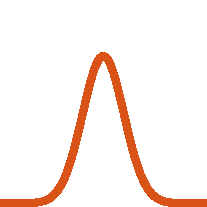
\includegraphics[height=.8cm]{distri}} + \dots + \raisebox{-1mm}{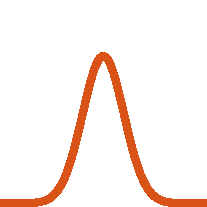
\includegraphics[height=.8cm]{distri}} &{ \approx \! \raisebox{-1mm}{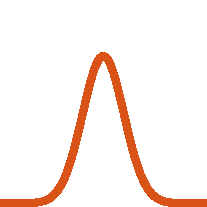
\includegraphics[height=.8cm]{distri}}}  \;{\raisebox{-0.5mm}{
\includegraphics[height=5mm]{check}}} \\[6pt]
 \ln {M} &=& \ln (M) &=  \ln (\raisebox{-1mm}{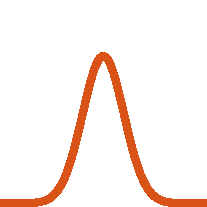
\includegraphics[height=.8cm]{distri}} ) &{ \approx \! \raisebox{-1mm}{
\includegraphics[height=.6cm]{log_gaussian}}}  \;{\raisebox{-0.5mm}{
\includegraphics[height=5mm]{check}}} \\[6pt]
 \ln \tilde{M} &=& \ln (\tilde{M}) &= \ln (\raisebox{-1mm}{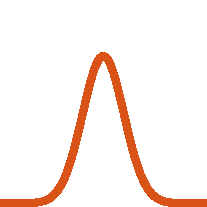
\includegraphics[height=.8cm]{distri}} ) &{ \approx \! \raisebox{-1mm}{
\includegraphics[height=.6cm]{log_gaussian}}}  \;{\raisebox{-0.5mm}{
\includegraphics[height=5mm]{check}}} \\[6pt]
\check{A} &=& \ln M - \ln \tilde{M} &= \raisebox{-1mm}{
\includegraphics[height=.6cm]{log_gaussian}} - \raisebox{-1mm}{
\includegraphics[height=.6cm]{log_gaussian}}  &{ \approx \! \raisebox{-1mm}{
\includegraphics[height=.6cm]{log_gaussian}}}  \;{\raisebox{-0.5mm}{
\includegraphics[height=5mm]{check}}} \\[6pt]
 A &=& \exp(\check{A}) &= \exp (\raisebox{-1mm}{
\includegraphics[height=.6cm]{log_gaussian}})  &{ \approx \! \raisebox{-1mm}{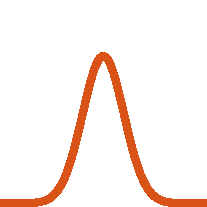
\includegraphics[height=.8cm]{distri}}}  \;{\raisebox{-0.5mm}{
\includegraphics[height=5mm]{check}}} \\[6pt]
\end{array}$\bigskip
\end{block}

\begin{block}{Epistemic uncertainty on classes using Remax}\vspace{0pt}\centering


\begin{figure}[h]
    \centering
    \begin{minipage}[b]{0.5\textwidth}
        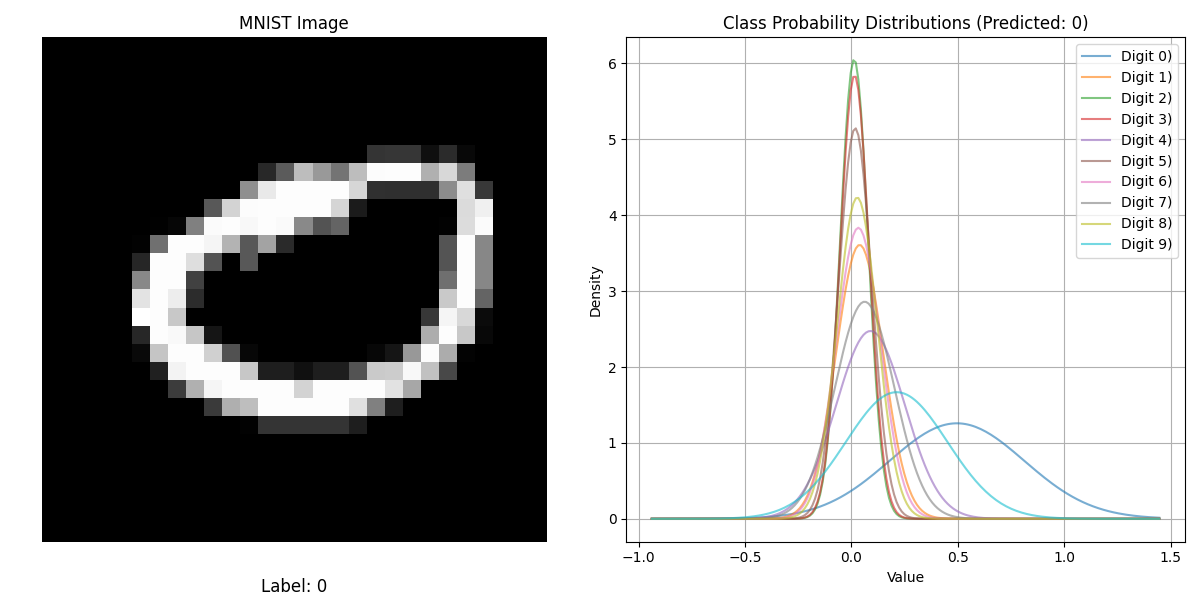
\includegraphics[width=\textwidth]{0}
        \caption*{0 predicted on MNIST.}
    \end{minipage}\hfill
    \begin{minipage}[b]{0.5\textwidth}
        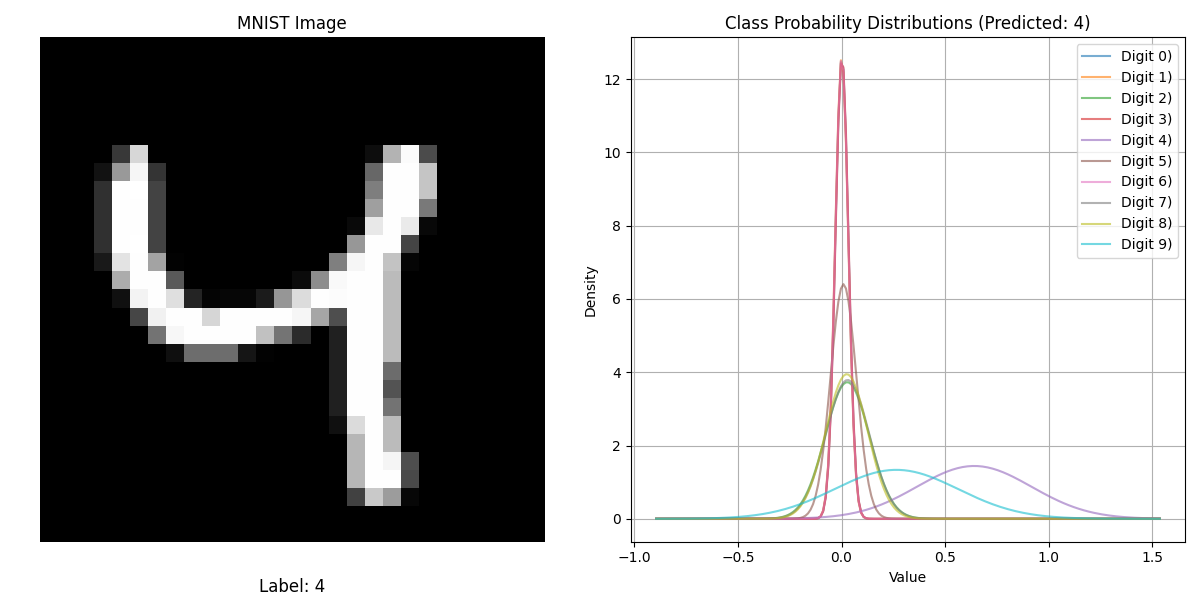
\includegraphics[width=\textwidth]{4}
        \caption*{4 predicted on MNIST.}
    \end{minipage}
\end{figure}

\begin{figure}[h]
    \centering
    \begin{minipage}[b]{0.5\textwidth}
        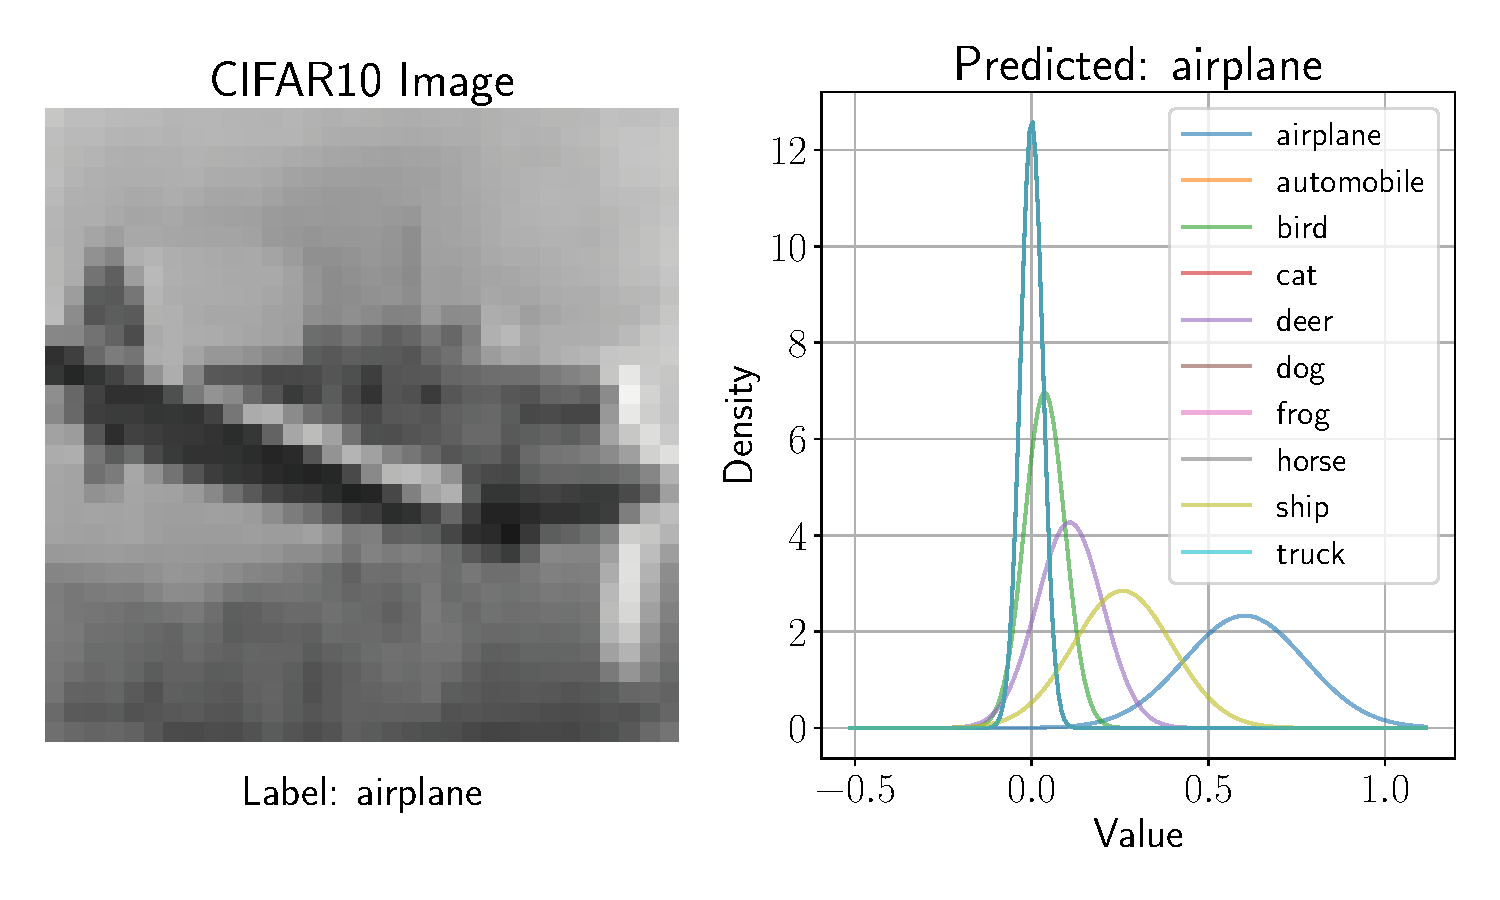
\includegraphics[width=\textwidth]{airplane}
        \caption*{Correct prediction on CIFAR10.}
    \end{minipage}\hfill
    \begin{minipage}[b]{0.5\textwidth}
        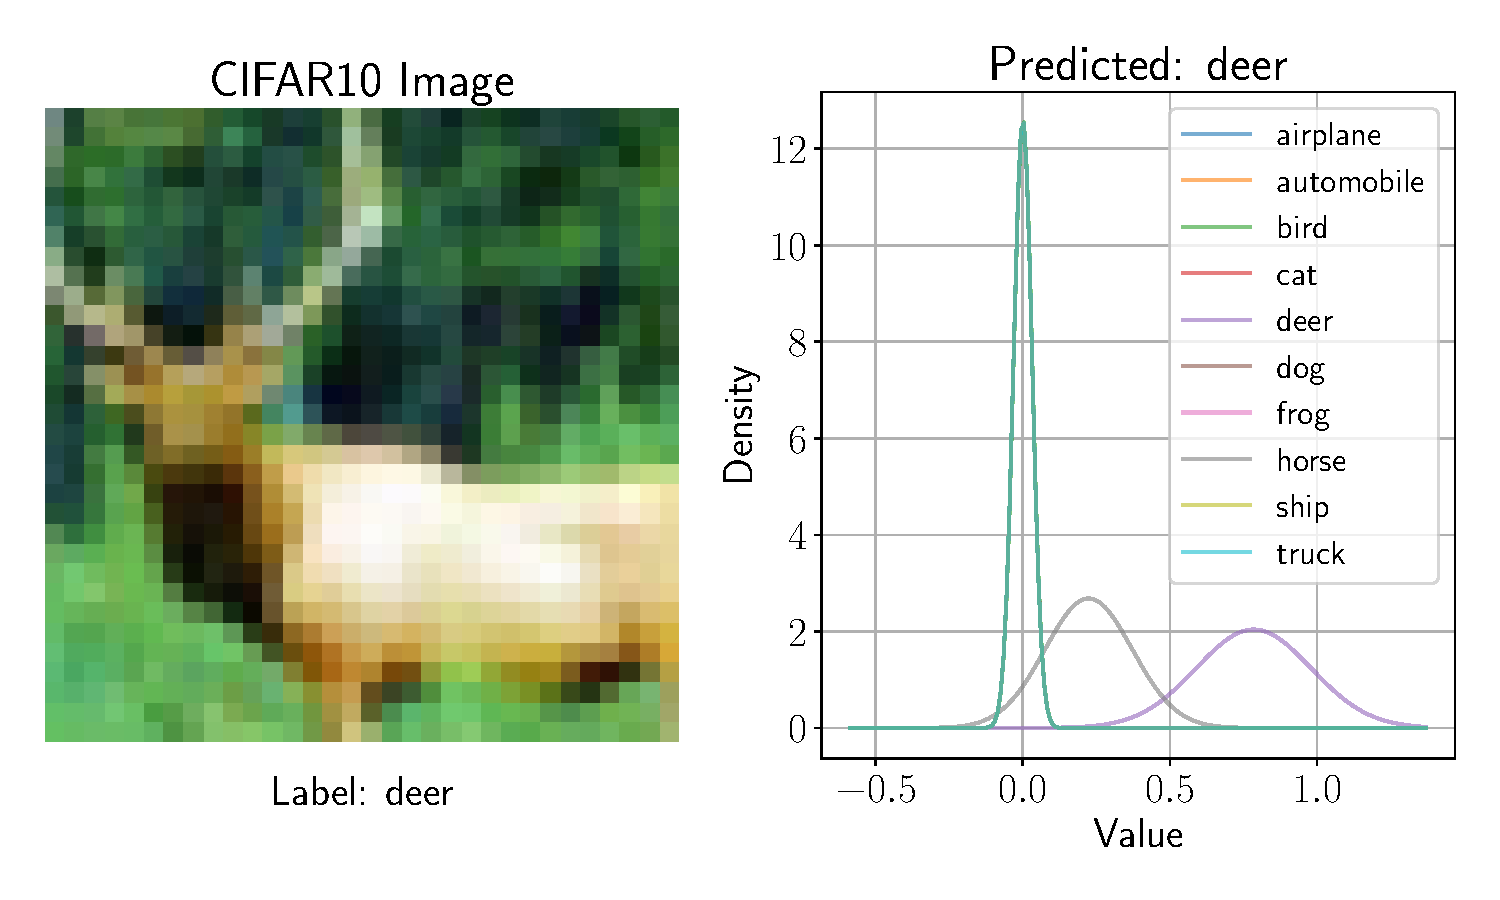
\includegraphics[width=\textwidth]{deer}
        \caption*{Correct prediction on CIFAR10.}
    \end{minipage}
\end{figure}

\begin{figure}[h]
    \centering
    \begin{minipage}[b]{0.5\textwidth}
        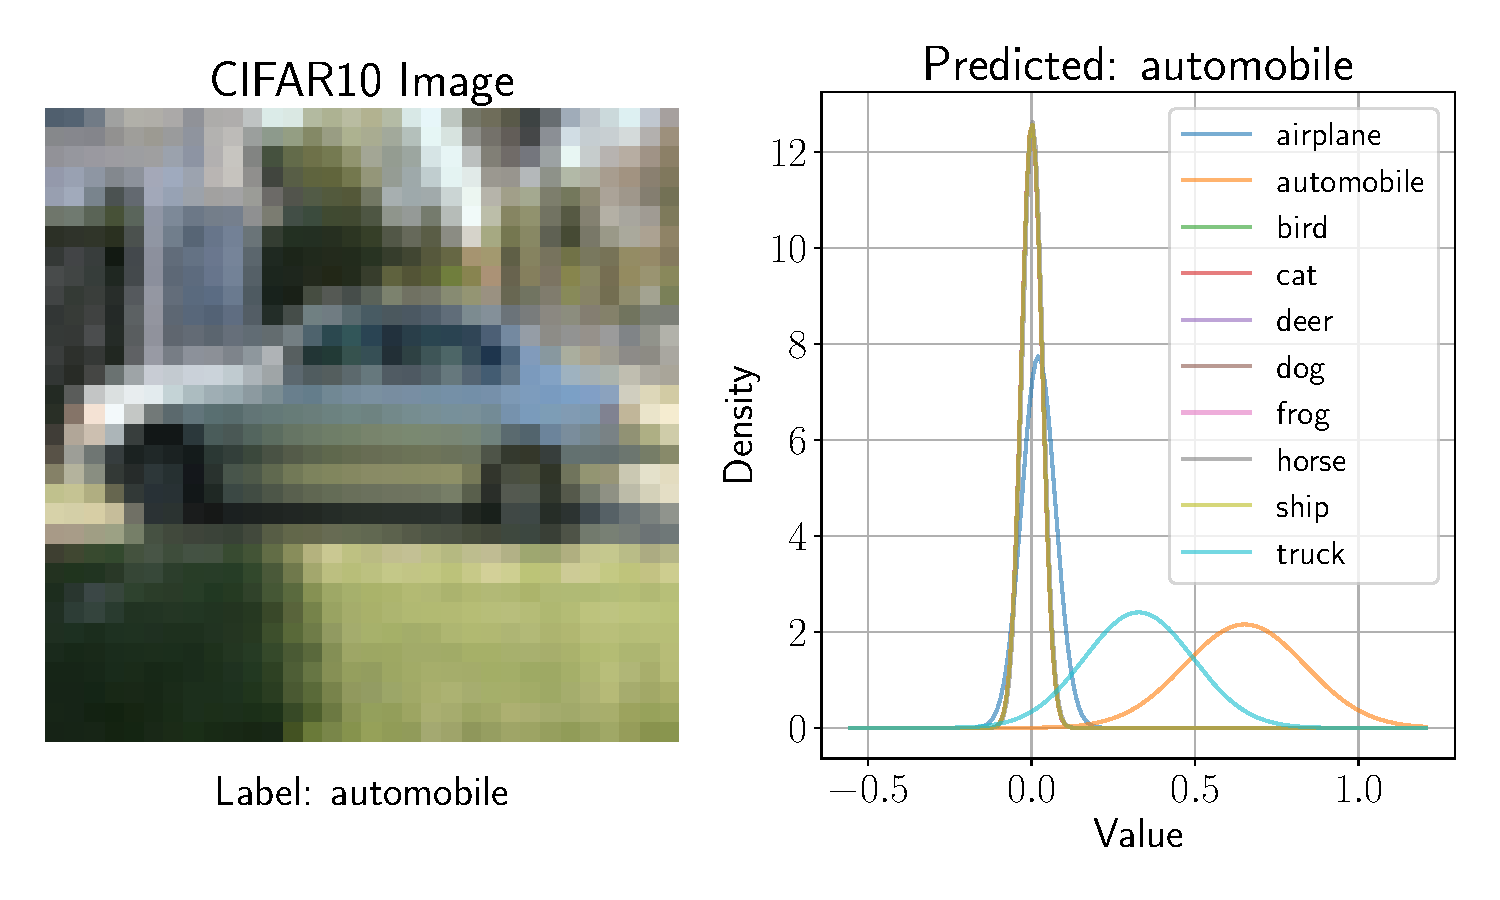
\includegraphics[width=\textwidth]{automobile}
        \caption*{Correct prediction on CIFAR10.}
    \end{minipage}\hfill
    \begin{minipage}[b]{0.5\textwidth}
        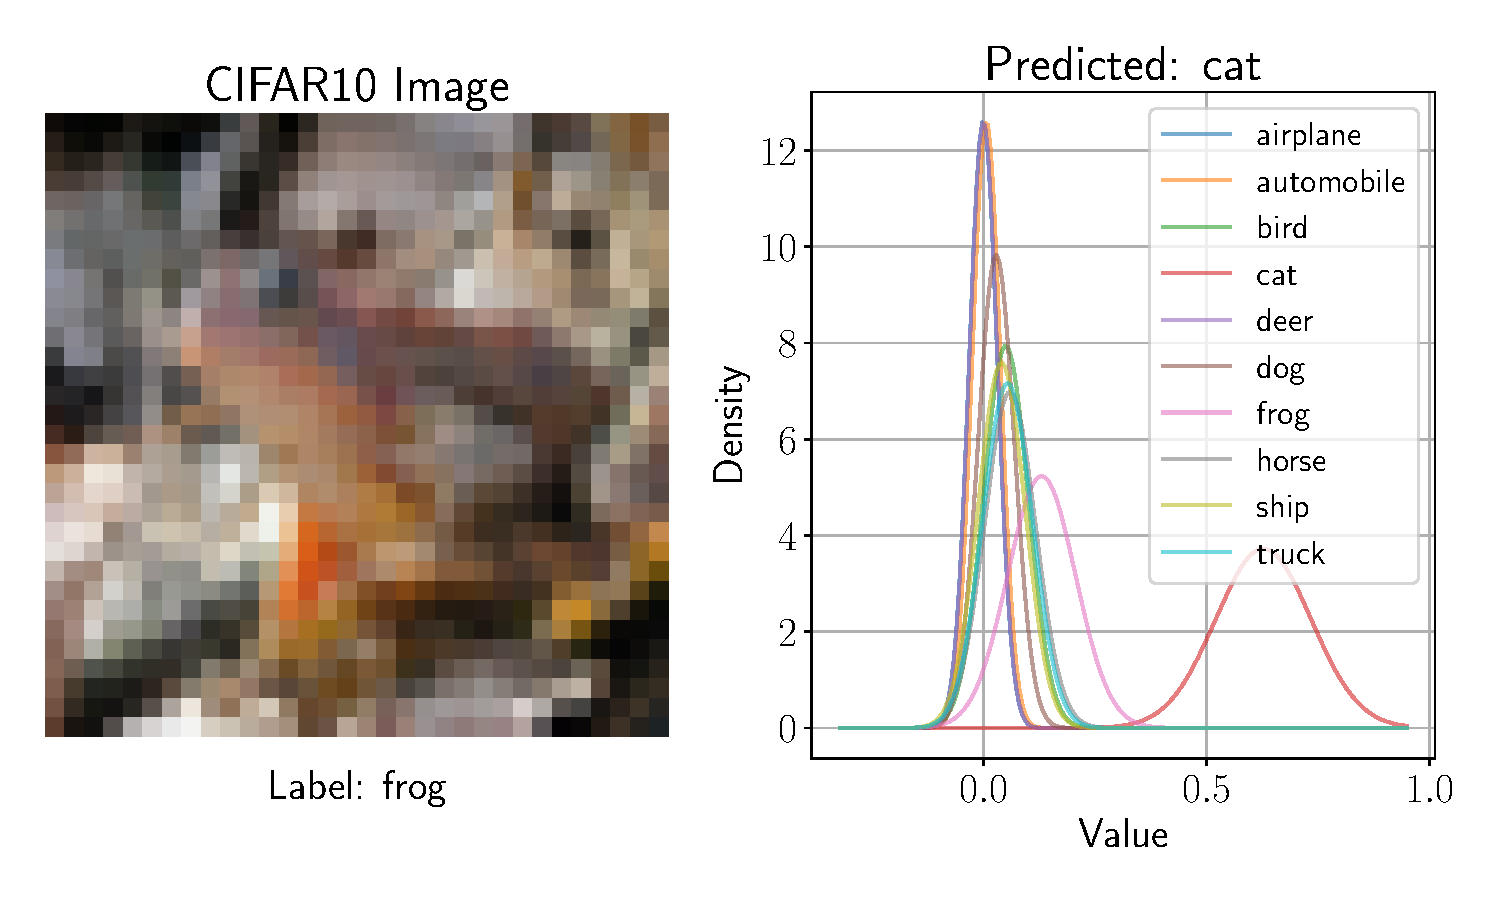
\includegraphics[width=\textwidth]{frog}
        \caption*{Wrong prediction on CIFAR10.}
    \end{minipage}
\end{figure}

\end{block}
\end{column}
%%%%%%%%%%
%%% Column 3
%%%%%%%%%%
\begin{column}[T]{.31\textwidth}

%% Key Results
\begin{block}{Key Results: TAGI-HRC vs. TAGI-Remax vs. Torch}
\centering
\begin{tabular}{lcc}
\toprule
Framework & Avg. Training Error & Avg. Test Error \\
\midrule
Torch      & 10.05 & 10.69 \\
TAGI-HRC       & 7.07  & \textbf{7.73} \\
TAGI-Remax & 7.14  & \textbf{7.78} \\
\bottomrule
\end{tabular}
\end{block}

%% Important Findings
\begin{block}{Important Findings}
\begin{itemize}
    \item \textbf{Batch Size:} TAGI excels with smaller batches, while Torch performs better with larger batches.
    \item \textbf{Network Depth:} TAGI maintains stability as depth increases, unlike Torch, which struggles without batch normalization.
    \item \textbf{Effect of $\sigma_v$:} Higher $\sigma_v$ values enhance TAGI's performance, especially in deeper networks.
    \item \textbf{Capacity Effect:} TAGI benefits more from increasing neurons/channels, showing improved generalization, while Torch fails to utilize additional capacity effectively.
    \item \textbf{Comparison of Implementations:} TAGI-HRC achieves better error rates overall, while TAGI-Remax shows higher stability but less frequent best-case performance.
    \item \textbf{Batch Normalization:} TAGI performs well even without batch normalization, handling deeper architectures (5+ layers) where Torch often diverges.
\end{itemize}
\end{block}

%% Figures and Tables (Side-by-Side)
\begin{block}{Ablation Study: Performance Comparisons and Capacity Effects}
\begin{figure}[h]
    \centering
    \begin{minipage}[b]{0.48\textwidth}
        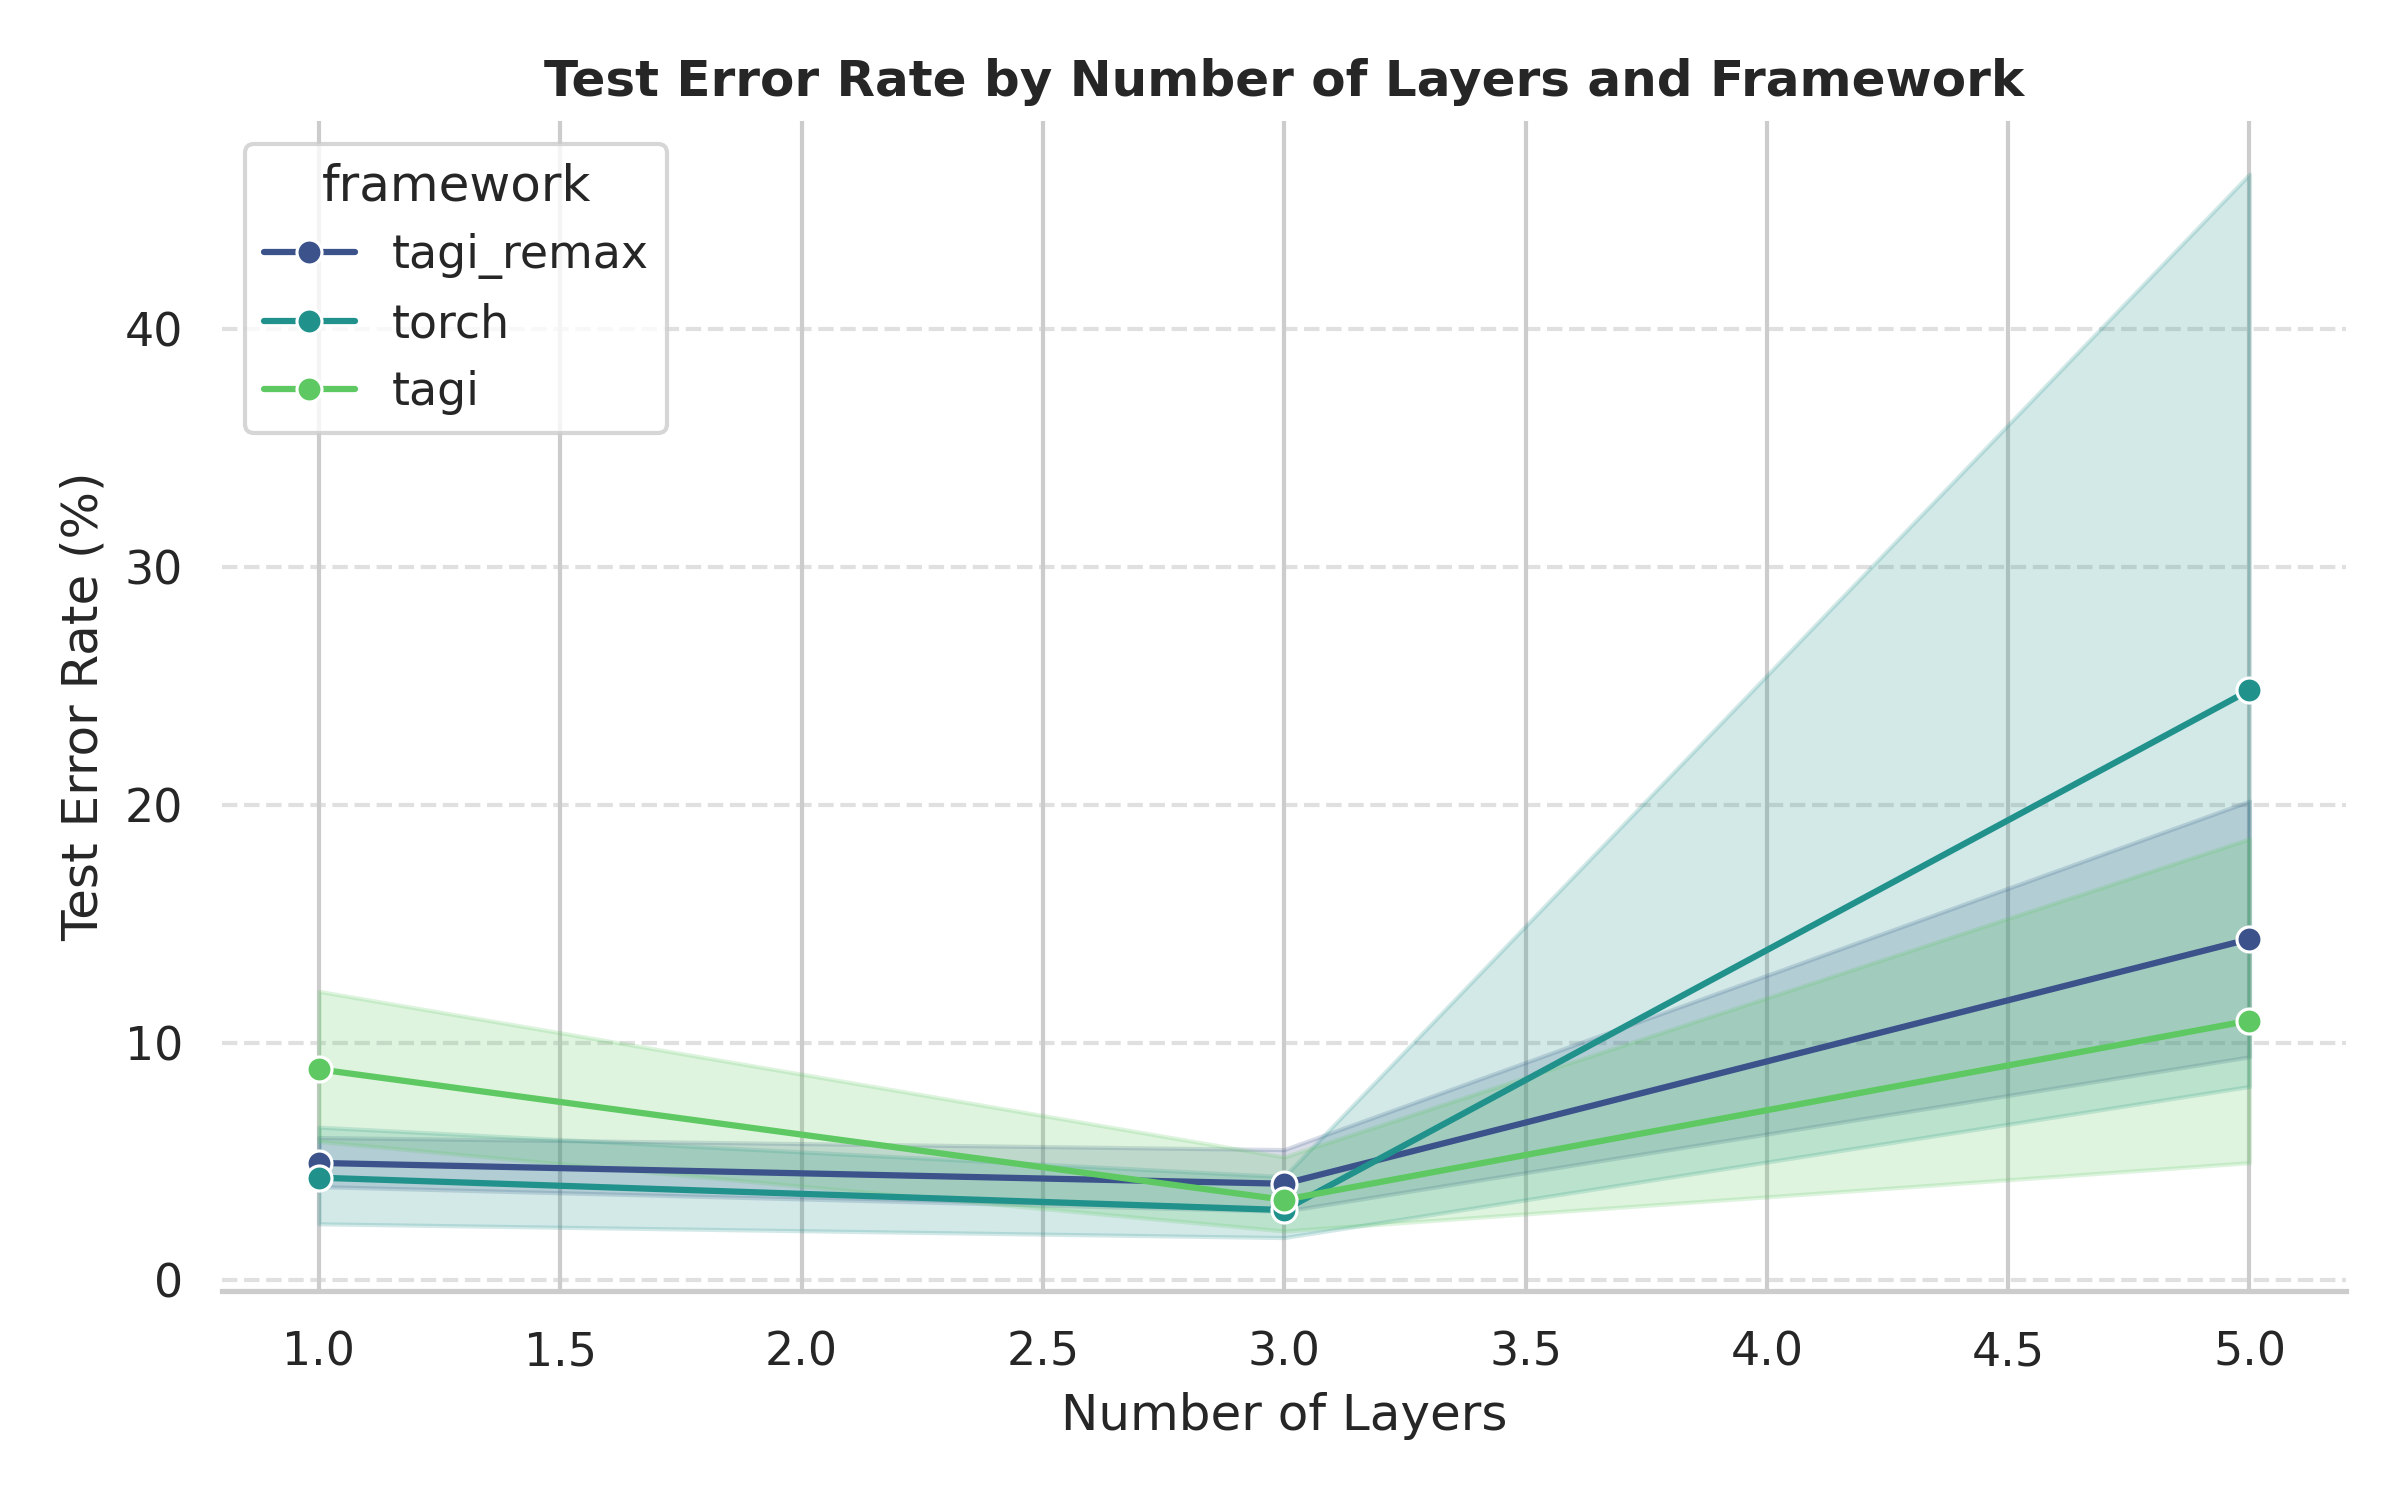
\includegraphics[width=\textwidth]{Figures/num_layers_test_error.png}
        \caption*{\textbf{Test Error vs Network Depth:} TAGI maintains low error rates, while Torch degrades significantly.}
    \end{minipage}\hfill
    \begin{minipage}[b]{0.48\textwidth}
        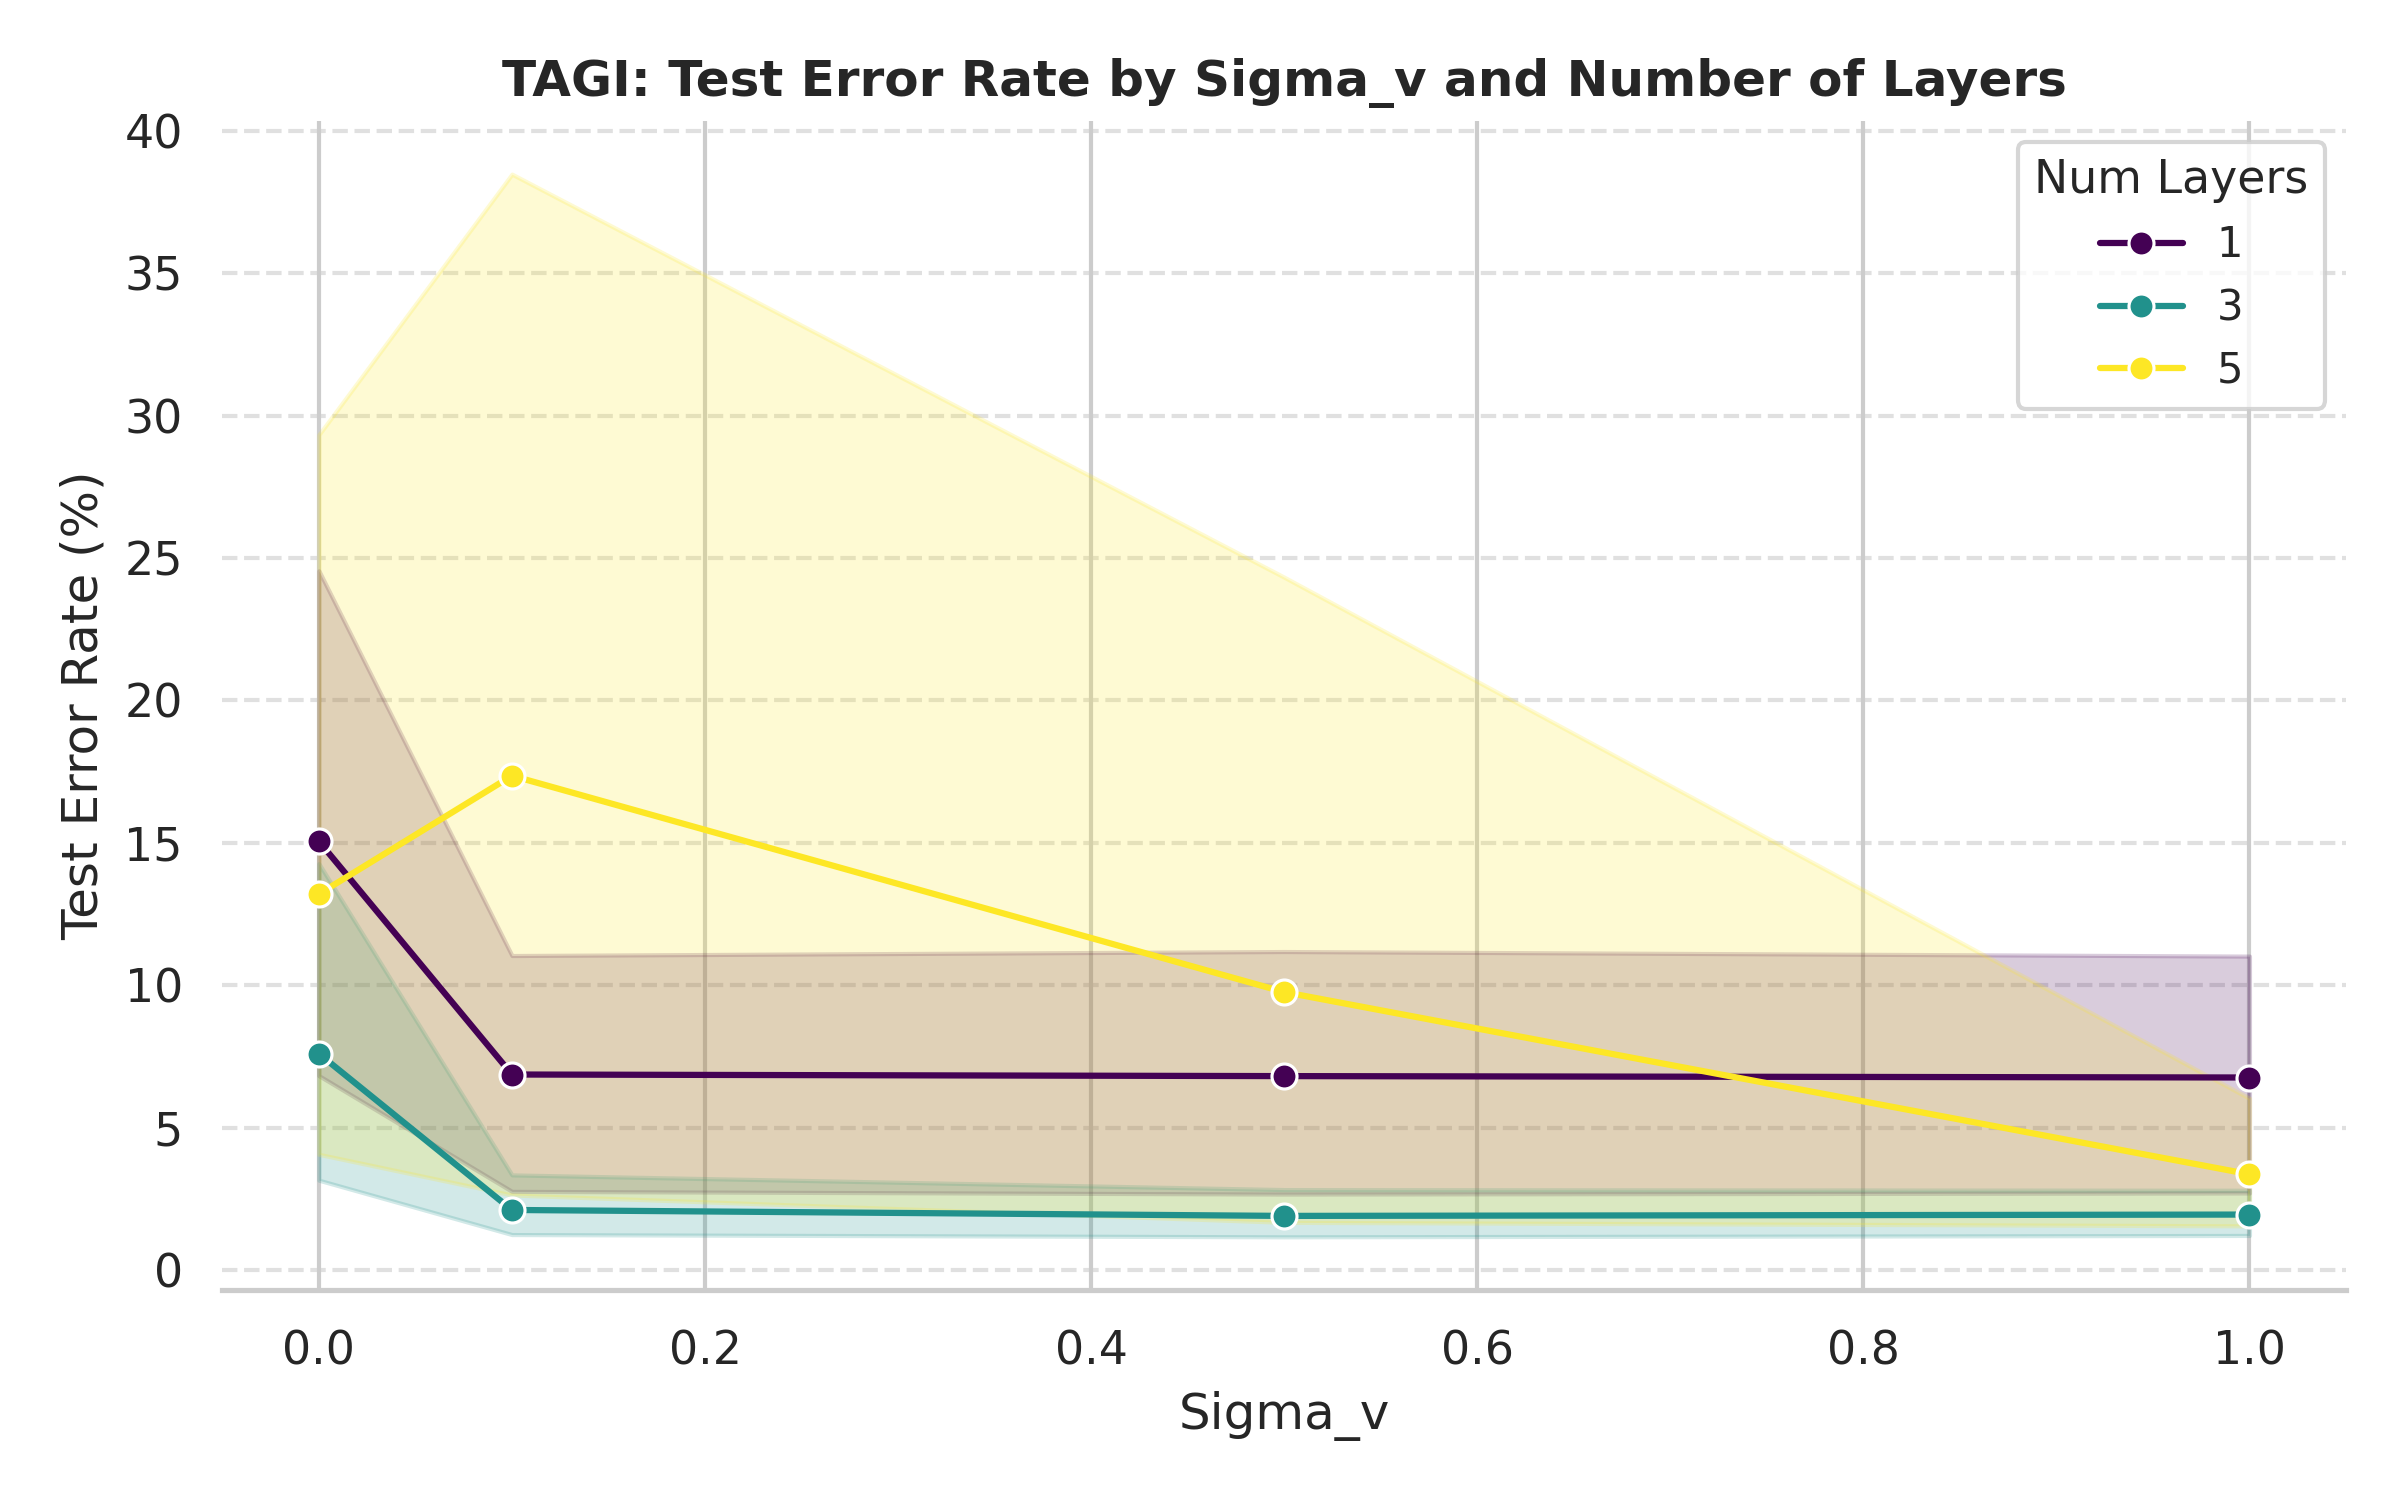
\includegraphics[width=\textwidth]{Figures/tagi_sigma_comparison.png}
        \caption*{\textbf{Impact of $\sigma_v$:} Higher $\sigma_v$ values improve TAGI's test error.}
    \end{minipage}
\end{figure}




\begin{columns}
\begin{column}{0.48\textwidth}
\centering
\begin{tabular}{lcccc}
\toprule
 & \multicolumn{2}{c}{Small Batch (16)} & \multicolumn{2}{c}{Large Batch (512)} \\
Framework & With BN & W.o BN & With BN & W.o BN \\
\midrule
Torch      & \textbf{1.35} & 31.20 & \textbf{1.06} & 16.22 \\
TAGI-HRC       & 1.97         & \textbf{1.74} & 4.11 & 15.99 \\
TAGI-Remax & 12.05         & 7.30         & 5.75 & \textbf{5.43} \\
\bottomrule
\end{tabular}
\end{column}
\begin{column}{0.48\textwidth}
\centering
\begin{tabular}{lcc}
\toprule
 & Small (32) & Large (512) \\
Framework & Neurons/layer & Neurons/layer \\
\midrule
Torch      & 7.03 &  7.32 \\
TAGI-HRC       & 13.58         &  \textbf{8.98} \\
TAGI-Remax &  9.25         &  \textbf{6.91} \\
\bottomrule
\end{tabular}
\end{column}
\end{columns}
\end{block}


%% cuTAGI
\begin{block}{py/cuTAGI -- Open-source Bayesian deep-learning framework}\vspace{0pt}\centering


\begin{columns}
\begin{column}{.35\textwidth}\centering\bigskip


\bigskip


\medskip



\includegraphics[width=115mm]{Figures/cupyTAGI.pdf}\\[20pt]


{\texttt{github\!.\!com/lhnguyen102/\!cuTAGI}}\\[20pt]
%{\LARGE\texttt{tagiml.com}}\\[20pt]
{\Large\texttt{\alert{ pip install pytagi}}}
\end{column}
%\begin{column}{.22\textwidth}\centering\vspace{-25pt}
%\includegraphics[width=120mm]{Figures/cutagi_example.pdf}
%\end{column}
\begin{column}{.6\textwidth}
\begin{itemize}
\item \alert{\bf Performance-Oriented Kernels} written in C++/CUDA from scratch, with pybind11 for a seamless integration. It allows running on CPU \& CUDA devices through a Python API.
\item \alert{\bf Broad Architecture Support} of the basic DNN layer including \emph{\color{darkblue}\bf Linear}, \emph{\color{cyan}\bf CNNs}, \emph{\color{blue}\bf Transposed CNNs}, \emph{\color{magenta}\bf LSTM}, \emph{\color{orange}\bf Average pooling}, \emph{\color{teal}\bf Batch} and \emph{\color{violet}\bf Layer normalization}, enabling the building of mainstream architectures such as \emph{Autoencoders}, \emph{Transformers}, \emph{Diffusion Models}, and \emph{GANs}.
\item \alert{\bf Model Building and Execution} currently supports sequential model building, with plans to introduce Eager Execution
\item \alert{\bf Open Platform} providing access to its entire codebase. 
\end{itemize}


\end{column}
\end{columns}
\end{block}%\bigskip
\vspace{-5mm}


 
%% cuTAGI
\begin{block}{TAGI-related references}\vspace{10pt}


\begin{columns}
\begin{column}{.15\textwidth}\centering

\includegraphics[width=30mm]{Figures/cuTAGI_refs_QR.pdf}\\[5pt]

\includegraphics[width=20mm]{Figures/IJF.jpg}\\[5pt]
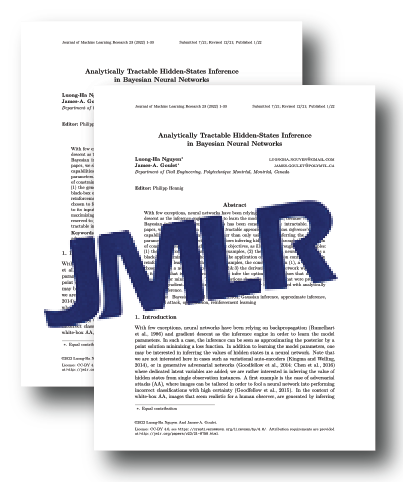
\includegraphics[width=22mm]{Figures/TAGI_AA_JMLR_2.png}
\end{column}\hspace{-20mm}


\begin{column}{.79\textwidth}
\begin{itemize}
%\item \emph{Coupling LSTM Neural Networks and SSM through Analytically Tractable Inference},\\(Vuong, Nguyen \& Goulet, International Journal of Forecasting, 2024)
\item \emph{\bf Analytically tractable hidden-states inference in Bayesian neural networks}\\ (Nguyen and Goulet. Journal-to-conference track, ICLR 2024)
\item \emph{Analytically tractable heteroscedastic uncertainty quantification in Bayesian neural networks for regression tasks}\\ (Deka, Nguyen \& Goulet. Neurocomputing, 2024)
\item \emph{\bf Tractable approximate Gaussian inference for Bayesian neural networks}\\ (Goulet, Nguyen, \& Amiri, JMLR, 2021)
%\item \emph{Analytically tractable inference in deep neural networks}\\ (Nguyen and Goulet. 2021)
%\item \emph{Analytically tractable Bayesian deep Q-Learning} (Nguyen and Goulet. 2021)
\end{itemize}
\end{column}
\end{columns}
\end{block}




\end{column}
%%%%%%%%%%%
%%%% Column 4
%%%%%%%%%%%
%\begin{column}[T]{.25\textwidth}
%\end{column}
\end{columns}
\end{frame}
\end{document}
